\documentclass[10pt,journal]{IEEEtran}
\usepackage{graphicx,booktabs,amsmath}
\usepackage[T1]{fontenc}
\usepackage{lmodern}
\begin{document}
\title{A 1.1-V Fully Differential OTA in the Supplied 180-nm Model}
\author{Three-pass design and simulation study}
\maketitle
\begin{abstract}
A ten-transistor OTA settles a 250-mV differential output step to within 0.5\% of its final value in 4.76 ns on the rising edge and 4.78 ns on the falling edge. Redesign raises loop gain by 7.63 dB and reduces nominal dissipation from 457 to 353 $\mu$W. The results are transistor-level schematic simulations with the supplied nominal 180-nm BSIM3 model. Process and mismatch sensitivities are reported with explicit perturbation assumptions.
\end{abstract}
\section{Introduction}
The objective is to meet the specified charge-transfer accuracy, speed, noise and stability at low quiescent power. The independent design was frozen before reading the supplied solution. A second pass compared the documented results, and a third applied headroom and compensation changes to the independent circuit. Both measured designs use the same 1.1-V supply and nominal 27$^\circ$C model.
\begin{table}[h]
\caption{Nominal results, independently measured in ngspice}
\centering
\begin{tabular}{@{}lll@{}}\toprule
Metric & Target & Revised OTA \\ \midrule
$C_s,C_f,C_L$ (each side) & 1,.25,.25 pF & as specified \\
Static step error & $\leq$0.5\% & 0.3974\% \\
Dynamic error, 10 ns$^a$ & $\leq$0.5\% & 0.0671\% \\
Dynamic error, 40 ns$^a$ & reported & 0.000031\% \\
3-dB output span & $\geq$0.5 V & $\pm$0.757 V \\
Output common mode & --- & 0.591 V \\
Input common-mode range & --- & 0.443--0.927 V \\
DC / LF loop gain & --- & 65.98 / 48.09 dB \\
Loop crossover & --- & 81.66 MHz \\
Differential phase margin & $\geq 60^\circ$ & $70.13^\circ$ \\
Rise / fall, 0.5\% band & $\leq$10 ns & 4.76 / 4.78 ns \\
Rise / fall, 1\% band & $\leq$10 ns & 4.50 / 4.50 ns \\
LF CMRR / PSRR & $\geq$60 dB & 95.08 / 103.69 dB \\
Offset sample $\sigma$, assumed$^b$ & --- & 2.00 mV \\
Differential output noise & $\leq$600 $\mu$V & 527.4 $\mu$V rms \\
Total static power & minimize & 353.5 $\mu$W \\ \bottomrule
\end{tabular}\\[3pt]
$^a$Worst edge, normalized to the ideal 250-mV step.\\
$^b$20 threshold-only samples. See Section~\ref{sec:mismatch}.
\end{table}
\section{Architecture and sizing}
A telescopic stack would consume voltage headroom. A folded input stage and class-AB output, as in the reference, would require additional bias branches. Our original design uses an NMOS differential pair, PMOS current-source loads, and a PMOS common-source output stage on each side. Each stage averages its two drain voltages through equal resistors and feeds that voltage to the load gates. Parallel sense capacitors improve the high-frequency common-mode path. There is one rail-tied reference current source. The tail mirror has a drawn 6:1 ratio.
\par In the independent version the tail device had 149 mV of $V_{DS}$ against a modeled $V_{DS,sat}$ of 169 mV. The revised bias uses a wider reference/tail pair and 17.2 $\mu$A of reference current. This gives 160 mV and 100 mV respectively. Wider PMOS input-stage loads raise the input-pair drains from 344 to 508 mV. Every nominal device now has $|V_{DS}|>|V_{DS,sat}|$. Each recovery in output resistance helps static accuracy.
\par The feedback factor without transistor parasitics is $\beta=C_f/(C_s+C_f)=0.2$. To limit finite-gain error to 0.5\%, $T_0\ge199$ is required. The independent loop reached only 40.46 dB. With the revised bias, the operating-point half-circuit gives $R_1=(g_{ds1}+g_{ds3}+1/R_1^s)^{-1}=58.3$ k$\Omega$ and analogously $R_2=32.7$ k$\Omega$, with $R_1^s=R_2^s=800$ k$\Omega$. Using $g_{m1}=0.752$ mS and $g_{m5}=1.395$ mS gives $A_0=g_{m1}R_1g_{m5}R_2=1995$ or 66.00 dB, versus 65.98 dB in simulation.
\par A first estimate $f_c=\beta g_{m1}/(2\pi C_c)$ gives 119.6 MHz. Gate overlap, input loading and finite second-stage bandwidth reduce the measured crossover to 81.66 MHz. The measured gain ratio $|T_0/A_0|=0.128$. The series resistor is raised from 0.62 to 4.15 k$\Omega$, above $1/g_{m5}=0.717$ k$\Omega$. This places the approximate compensation zero in the left half plane at 232 MHz and increases phase margin. Reference, input stage and output stage draw 18.92, 102.73 and 231.84 $\mu$W. Passive common-mode sensing has zero nominal DC drop across its resistors.
\section{Reference comparison}
The reference report describes a folded cascode, class-AB output and mixed compensation. It reports 312.78 MHz and $75.66^\circ$ in its stability plot, about 2 ns settling, 599 $\mu$V rms noise and 1.32 mW. Its summary table gives $<0.001\%$ static error, whereas its waveform annotation states below one part in a thousand. No runnable reference netlist was supplied. These are reported results under the course design context. The reference motivated checking stage gain, output drive and phase margin together. The revised circuit uses its own dimensions and saves 22.6\% power versus the independent version, with noise increasing from 481.2 to 527.4 $\mu$V.
\clearpage
\onecolumn
\section{Circuit and measurement}
\begin{center}
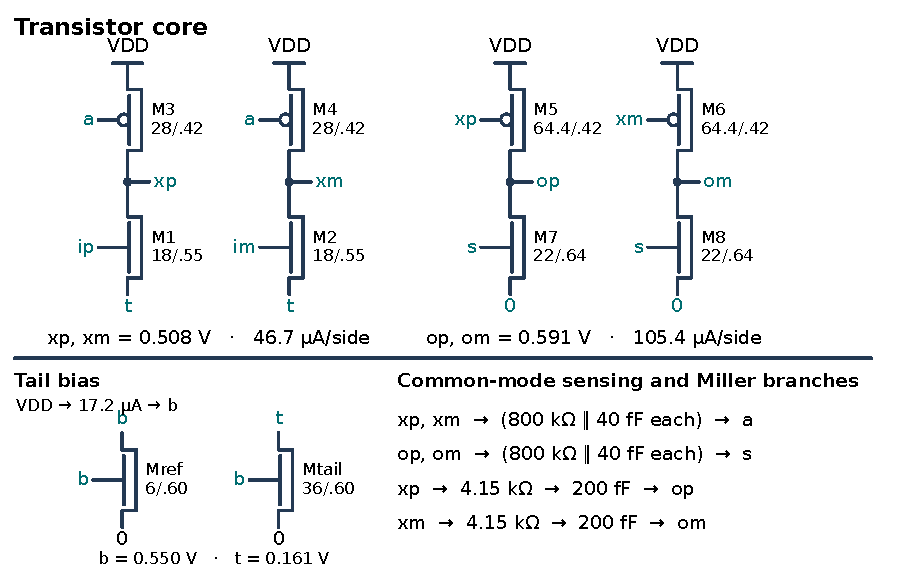
\includegraphics[width=.88\textwidth]{schematic.pdf}\\
Fig. 1. Revised schematic. Common net labels denote connections. NMOS bodies connect to ground and PMOS bodies to VDD. The two PMOS drains at the intermediate nodes share the average gate voltage $a$. The two output sinks share $s$.
\end{center}
\begin{center}
\begin{tabular}{@{}lrrrr@{}}
\toprule Devices & Drawn $W/L$ ($\mu$m/$\mu$m) & $I_D$ ($\mu$A each) & $|V_{DS}|$ (mV) & $|V_{DS,sat}|$ (mV) \\ \midrule
Reference & 6 / 0.60 & 17.2 & 550 & 102 \\
Tail & 36 / 0.60 & 93.4 & 160 & 100 \\
M1, M2 & 18 / 0.55 & 46.7 & 346 & 97 \\
M3, M4 & 28 / 0.42 & 46.7 & 591 & 127 \\
M5, M6 & 64.4 / 0.42 & 105.4 & 508 & 127 \\
M7, M8 & 22 / 0.64 & 105.4 & 589 & 130 \\ \bottomrule
\end{tabular}
\end{center}
The simulator reads both supplied BSIM3v3.1 cards after translation of the Spectre headers. The supplied $X_W=-10$ nm and $X_L=0$ are applied to the instance dimensions. Rectangular source and drain diffusions extend 0.25 $\mu$m on each side. The results include device-model parasitics. No extracted interconnect or measured silicon data are available.
\par For the differential loop, split the gates from the two summing nodes and measure both columns of their differential admittance matrix at the operating point. Each port uses complementary half-volt AC drives. Reconnecting the ports imposes equal voltage and zero summed current. Normalizing the resulting characteristic equation by $Y_{11}+Y_{22}$ gives $1+T$, where $T=(Y_{12}+Y_{21})/(Y_{11}+Y_{22})$. This keeps output loading and both reverse and forward transfer terms. The table uses 1 kHz for the flat low-frequency value. Rejection is $20\log_{10}|A_{DM}/A_{CM,SE}|$ or $20\log_{10}|A_{DM}/A_{VDD,SE}|$, with a single-ended output for the disturbance and 450 fF on each output. The large-signal sweep measures $V_{od}/V_{id}$, then interpolates both contiguous $-3$ dB crossings.
\par The testbench uses $V_{IC}=0.75$ V, complementary 31.25-mV input steps, 10-ps edges, 25-ns delay, 50-ns high duration and 100-ns period. Each 1-GH DC feed in the revised bench is realized by a scaled 1-H coil: voltage and reflected-current factors of $10^{-3}$ and $10^{-6}$ give the specified impedance. This avoids poor conditioning in the direct 1-GH inductor stamp. The initial direct-coil experiment and its repeat agree to less than 0.001 ns on nominal settling. Testbench sources and coils are external to the OTA.
\clearpage
\section{Nominal frequency and time responses}
\begin{center}
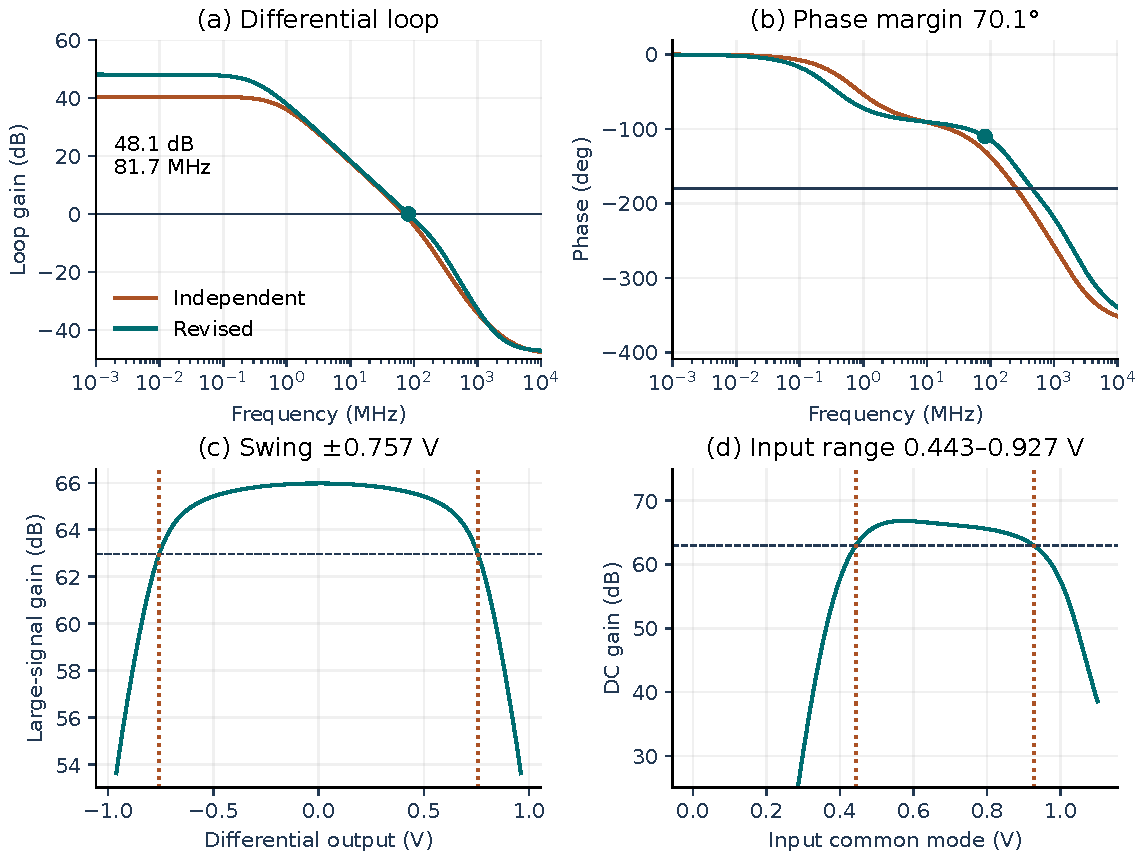
\includegraphics[width=.76\textwidth]{frequency.pdf}\\
Fig. 2. Differential loop gain and phase, 3-dB output swing and input common-mode gain.
\end{center}
\begin{center}
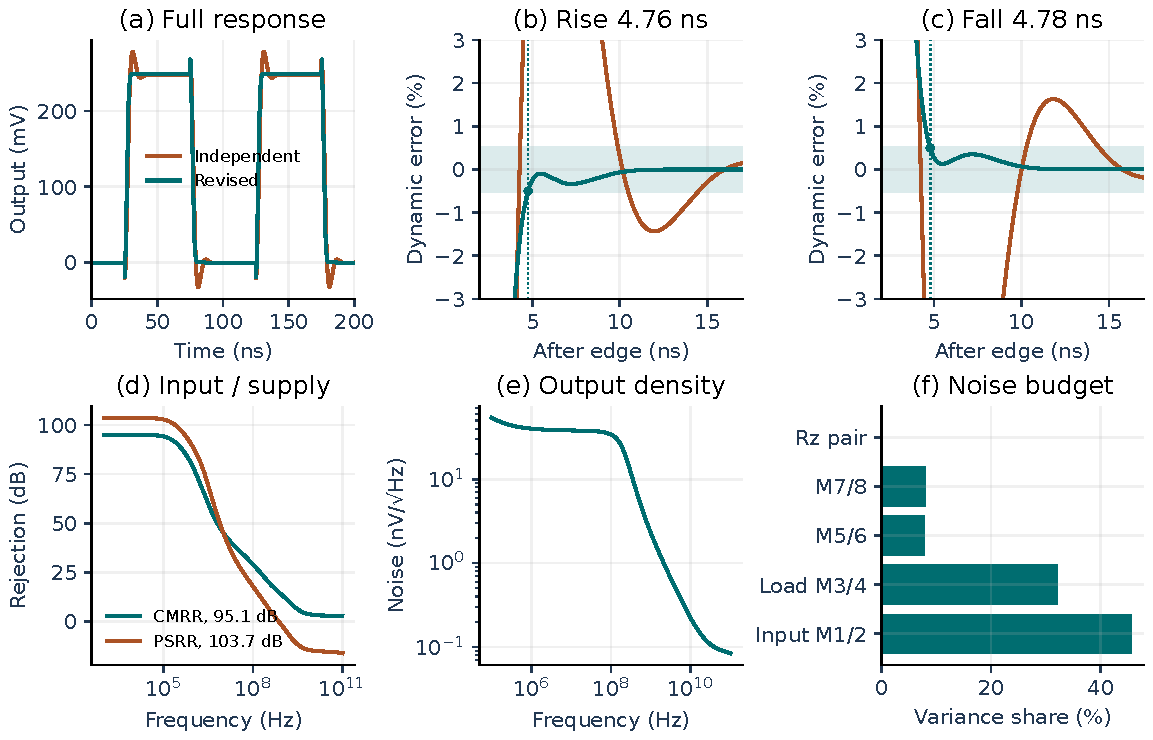
\includegraphics[width=.81\textwidth]{time_noise.pdf}\\
Fig. 3. Transient response, rejection and noise. Shading shows the $\pm0.5\%$ dynamic error band. Device groups show integrated variance, with all components in the data archive.
\end{center}
The two static levels are averaged before the edge and 48--49 ns after it. Static error compares their separation with 250 mV. Dynamic error compares the instantaneous output with the attained plateau. Settling is the last crossing into the band through 49 ns, interpolated from the 10-ps or finer samples. Against the ideal output at 10 ns, the rising and falling errors are 0.464\% and 0.067\% respectively. The stricter 0.5\% band is used throughout alongside the handout's 1\% convention. Output noise is integrated from 100 kHz to 100 GHz in closed loop.
\clearpage
\section{Voltage, temperature and statistical sensitivity}\label{sec:var}
The supplied file contains nominal N/P models only. TT uses these cards at both supply voltages and three temperatures. In each illustrative fast/slow polarity, mobility changes by $\pm12\%$ and threshold magnitude by $\mp25$ mV. The first letter labels NMOS. Table II gives all 30 combinations and both 0.5\% settling times. The six TT rows are voltage/temperature sweeps of the supplied model.
\begin{center}
TABLE II. Measured response for the nominal and illustrative process cases.\\[4pt]
\begin{tabular}{@{}lrrrrrrrr@{}}\toprule
N/P & VDD (V) & Temp. ($^\circ$C) & $A_{DM}$ (dB) & $T_0$ (dB) & $f_c$ (MHz) & PM ($^\circ$) & Rise (ns) & Fall (ns) \\ \midrule
TT & 1.1 & -25 & 66.83 & 48.80 & 97.41 & 71.34 & 7.40 & 7.40 \\
TT & 1.1 & 27 & 65.98 & 48.09 & 81.66 & 70.13 & 4.76 & 4.78 \\
TT & 1.1 & 85 & 64.94 & 47.22 & 68.32 & 68.92 & 8.20 & 8.16 \\
TT & 1.2 & -25 & 67.53 & 49.40 & 98.24 & 71.57 & 7.39 & 7.40 \\
TT & 1.2 & 27 & 66.90 & 48.87 & 82.45 & 70.30 & 4.85 & 4.88 \\
TT & 1.2 & 85 & 66.11 & 48.21 & 69.09 & 69.01 & 7.93 & 7.89 \\
FF & 1.1 & -25 & 67.06 & 49.03 & 103.28 & 72.25 & 7.25 & 7.25 \\
FF & 1.1 & 27 & 66.24 & 48.34 & 86.54 & 71.03 & 7.56 & 7.58 \\
FF & 1.1 & 85 & 65.19 & 47.46 & 72.63 & 69.79 & 5.19 & 5.19 \\
FF & 1.2 & -25 & 67.66 & 49.54 & 104.08 & 72.51 & 7.24 & 7.24 \\
FF & 1.2 & 27 & 67.04 & 49.02 & 87.29 & 71.23 & 7.62 & 7.64 \\
FF & 1.2 & 85 & 66.22 & 48.33 & 73.36 & 69.91 & 5.20 & 5.21 \\
SS & 1.1 & -25 & 66.51 & 48.49 & 90.96 & 70.31 & 7.41 & 7.43 \\
SS & 1.1 & 27 & 65.65 & 47.78 & 76.03 & 69.11 & 6.66 & 6.60 \\
SS & 1.1 & 85 & 64.68 & 46.98 & 62.92 & 67.91 & 9.84 & 9.81 \\
SS & 1.2 & -25 & 67.33 & 49.19 & 91.81 & 70.52 & 7.46 & 7.47 \\
SS & 1.2 & 27 & 66.71 & 48.67 & 76.86 & 69.25 & 6.28 & 6.20 \\
SS & 1.2 & 85 & 66.00 & 48.08 & 63.73 & 67.97 & 9.62 & 9.60 \\
SF & 1.1 & -25 & 66.95 & 48.98 & 93.80 & 73.11 & 7.69 & 7.69 \\
SF & 1.1 & 27 & 66.12 & 48.27 & 78.26 & 71.76 & 7.78 & 7.81 \\
SF & 1.1 & 85 & 65.16 & 47.44 & 64.65 & 70.34 & 6.09 & 6.09 \\
SF & 1.2 & -25 & 67.58 & 49.54 & 94.54 & 73.38 & 7.69 & 7.70 \\
SF & 1.2 & 27 & 66.94 & 49.00 & 78.96 & 71.99 & 7.93 & 7.94 \\
SF & 1.2 & 85 & 66.16 & 48.33 & 65.33 & 70.51 & 6.14 & 6.15 \\
FS & 1.1 & -25 & 66.45 & 48.43 & 99.71 & 69.40 & 7.25 & 7.26 \\
FS & 1.1 & 27 & 65.46 & 47.63 & 83.69 & 68.32 & 6.29 & 6.25 \\
FS & 1.1 & 85 & 64.18 & 46.59 & 70.28 & 67.33 & 8.75 & 8.72 \\
FS & 1.2 & -25 & 67.34 & 49.14 & 100.69 & 69.56 & 7.25 & 7.25 \\
FS & 1.2 & 27 & 66.69 & 48.60 & 84.67 & 68.38 & 6.10 & 6.06 \\
FS & 1.2 & 85 & 65.86 & 47.93 & 71.31 & 67.24 & 8.57 & 8.55 \\
\bottomrule\end{tabular}
\end{center}
\clearpage
\section{Mismatch sensitivity}\label{sec:mismatch}
For mismatch, each transistor receives an independent Gaussian threshold perturbation with explicitly assumed standard deviation $3\;\mathrm{mV}\,\mu\mathrm{m}/\sqrt{WL}$. A unity differential DC servo finds the input null while holding the common mode fixed. The trim is then held during AC and transient runs. Twenty independent draws (seeds 101--120) give a sample offset standard deviation of 2.00 mV. A central-difference linearization of all ten device thresholds gives 1.70 mV. The sample gain, crossover and phase-margin ranges are 65.86--66.06 dB, 79.14--85.50 MHz and 69.79--70.39 degrees. The model file supplies neither measured mismatch coefficients nor foundry process sections.
\begin{center}
TABLE III. Independent threshold perturbations at 1.1 V and 27$^\circ$C.\\[4pt]
\begin{tabular}{@{}rrrrrrr@{}}\toprule
Seed & Input null (mV) & $A_{DM}$ (dB) & $f_c$ (MHz) & PM ($^\circ$) & Rise (ns) & Fall (ns) \\ \midrule
101 & -0.64 & 65.96 & 81.83 & 70.30 & 4.86 & 4.90 \\
102 & 0.94 & 65.98 & 81.32 & 70.15 & 4.75 & 4.86 \\
103 & 3.73 & 65.90 & 83.91 & 70.25 & 4.71 & 4.73 \\
104 & -0.66 & 65.95 & 82.21 & 70.28 & 4.83 & 4.85 \\
105 & 0.96 & 66.01 & 80.81 & 70.04 & 4.76 & 4.79 \\
106 & 2.42 & 65.93 & 82.77 & 70.31 & 4.86 & 4.81 \\
107 & -3.25 & 65.91 & 83.36 & 70.39 & 4.83 & 4.93 \\
108 & 2.78 & 65.86 & 85.50 & 70.11 & 4.50 & 6.82 \\
109 & 1.47 & 65.97 & 82.11 & 70.04 & 4.68 & 4.70 \\
110 & 0.19 & 65.95 & 82.08 & 70.38 & 4.94 & 4.94 \\
111 & -0.94 & 66.00 & 81.60 & 69.97 & 4.66 & 4.71 \\
112 & -3.03 & 66.06 & 79.14 & 69.79 & 4.71 & 4.80 \\
113 & 0.98 & 65.92 & 83.52 & 70.13 & 4.62 & 4.69 \\
114 & -0.94 & 66.03 & 80.25 & 69.89 & 4.73 & 4.73 \\
115 & -0.90 & 65.88 & 84.28 & 70.37 & 6.87 & 7.02 \\
116 & 1.44 & 66.02 & 80.65 & 69.92 & 4.70 & 4.74 \\
117 & -2.51 & 65.98 & 81.23 & 70.22 & 4.84 & 4.88 \\
118 & 2.44 & 66.01 & 80.65 & 70.03 & 4.78 & 4.77 \\
119 & -0.69 & 66.04 & 79.51 & 69.98 & 4.82 & 4.82 \\
120 & 2.75 & 66.02 & 80.24 & 70.02 & 4.81 & 4.78 \\
\bottomrule\end{tabular}
\end{center}
\begin{center}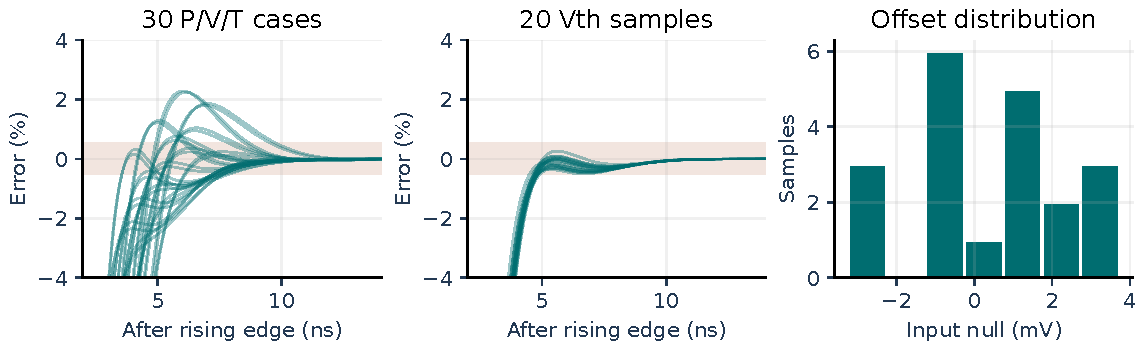
\includegraphics[width=.98\textwidth]{variation.pdf}\\
Fig. 4. Rising-edge response families and input-offset distribution. The archive preserves full 200-ns waveforms and sample-by-sample metrics.
\end{center}
\section{Conclusion}
The revised 180-nm schematic meets the nominal electrical thresholds. The slow/slow illustrative case at 1.1 V and 85$^\circ$C reaches the 0.5\% band in 9.84 ns, leaving little timing margin. Course-PDK process and statistical sign-off require the corresponding characterized models.
\end{document}
